% =====================================================================
% Relatório - Prática 3: Oscilações livres, amortecidas e forçadas
% Versão em arquivo único (prévia). Gerado a partir de main.tex,
% config/preambulo.tex e pags/*.tex; a única dependência externa é
% a imagem pags/imagens/usp-logo-0.png.
% =====================================================================
\documentclass[12pt, a4paper]{article}

% ======================== config/preambulo.tex ========================
\PassOptionsToPackage{table, dvipsnames}{xcolor}
\usepackage{xcolor}
\usepackage[utf8]{inputenc}
\usepackage[T1]{fontenc}
\usepackage[brazilian]{babel}

% ---------------------------------------------------------------
% Fonte, espaçamento e margens (ABNT NBR 14724)
% ---------------------------------------------------------------
\usepackage{mathptmx}
\usepackage{setspace}
\usepackage{indentfirst}
\onehalfspacing
\setlength{\parindent}{1.25cm}
\setlength{\emergencystretch}{2em}

\usepackage{geometry}
\geometry{
    a4paper,
    left=3cm,
    top=3cm,
    right=2cm,
    bottom=2cm
}

% ---------------------------------------------------------------
% Numeração de páginas no canto superior direito (ABNT NBR 14724)
% ---------------------------------------------------------------
\usepackage{fancyhdr}
\fancypagestyle{abnt}{%
    \fancyhf{}%
    \fancyhead[R]{\small\thepage}%
    \renewcommand{\headrulewidth}{0pt}%
}
\setlength{\headheight}{15pt}

% ---------------------------------------------------------------
% Matemática e unidades
% ---------------------------------------------------------------
\usepackage{amsmath}
\usepackage{amsfonts}
\usepackage{amssymb}
\usepackage{siunitx}
\sisetup{
    output-decimal-marker = {,},
    per-mode = symbol,
    separate-uncertainty = true
}
% unidade em texto reto, com espaço fino: $10\un{s}$
\newcommand{\un}[1]{\,\mathrm{#1}}
% citação numérica (ABNT NBR 10520, sistema numérico)
\newcommand{\cita}[1]{\textsuperscript{[#1]}}

% ---------------------------------------------------------------
% Figuras, tabelas e legendas (título acima, fonte abaixo)
% ---------------------------------------------------------------
\usepackage{graphicx}
\usepackage{float}
\usepackage{caption}
\captionsetup{
    labelsep = endash,
    justification = centering,
    font = {small, singlespacing},
    skip = 4pt
}
\usepackage{subcaption}
\usepackage{booktabs}
\usepackage{array}
\usepackage{multirow}
\newcommand{\fonte}[1]{\par\vspace{2pt}{\footnotesize Fonte: #1}}

\usepackage[
    colorlinks=true,
    linkcolor=black,
    citecolor=black,
    urlcolor=black
]{hyperref}

\graphicspath{{./pags/imagens/}}


\begin{document}

% ======================== pags/0-Capa.tex ========================
\begin{titlepage}
    \centering 
    \vspace*{-2cm}
    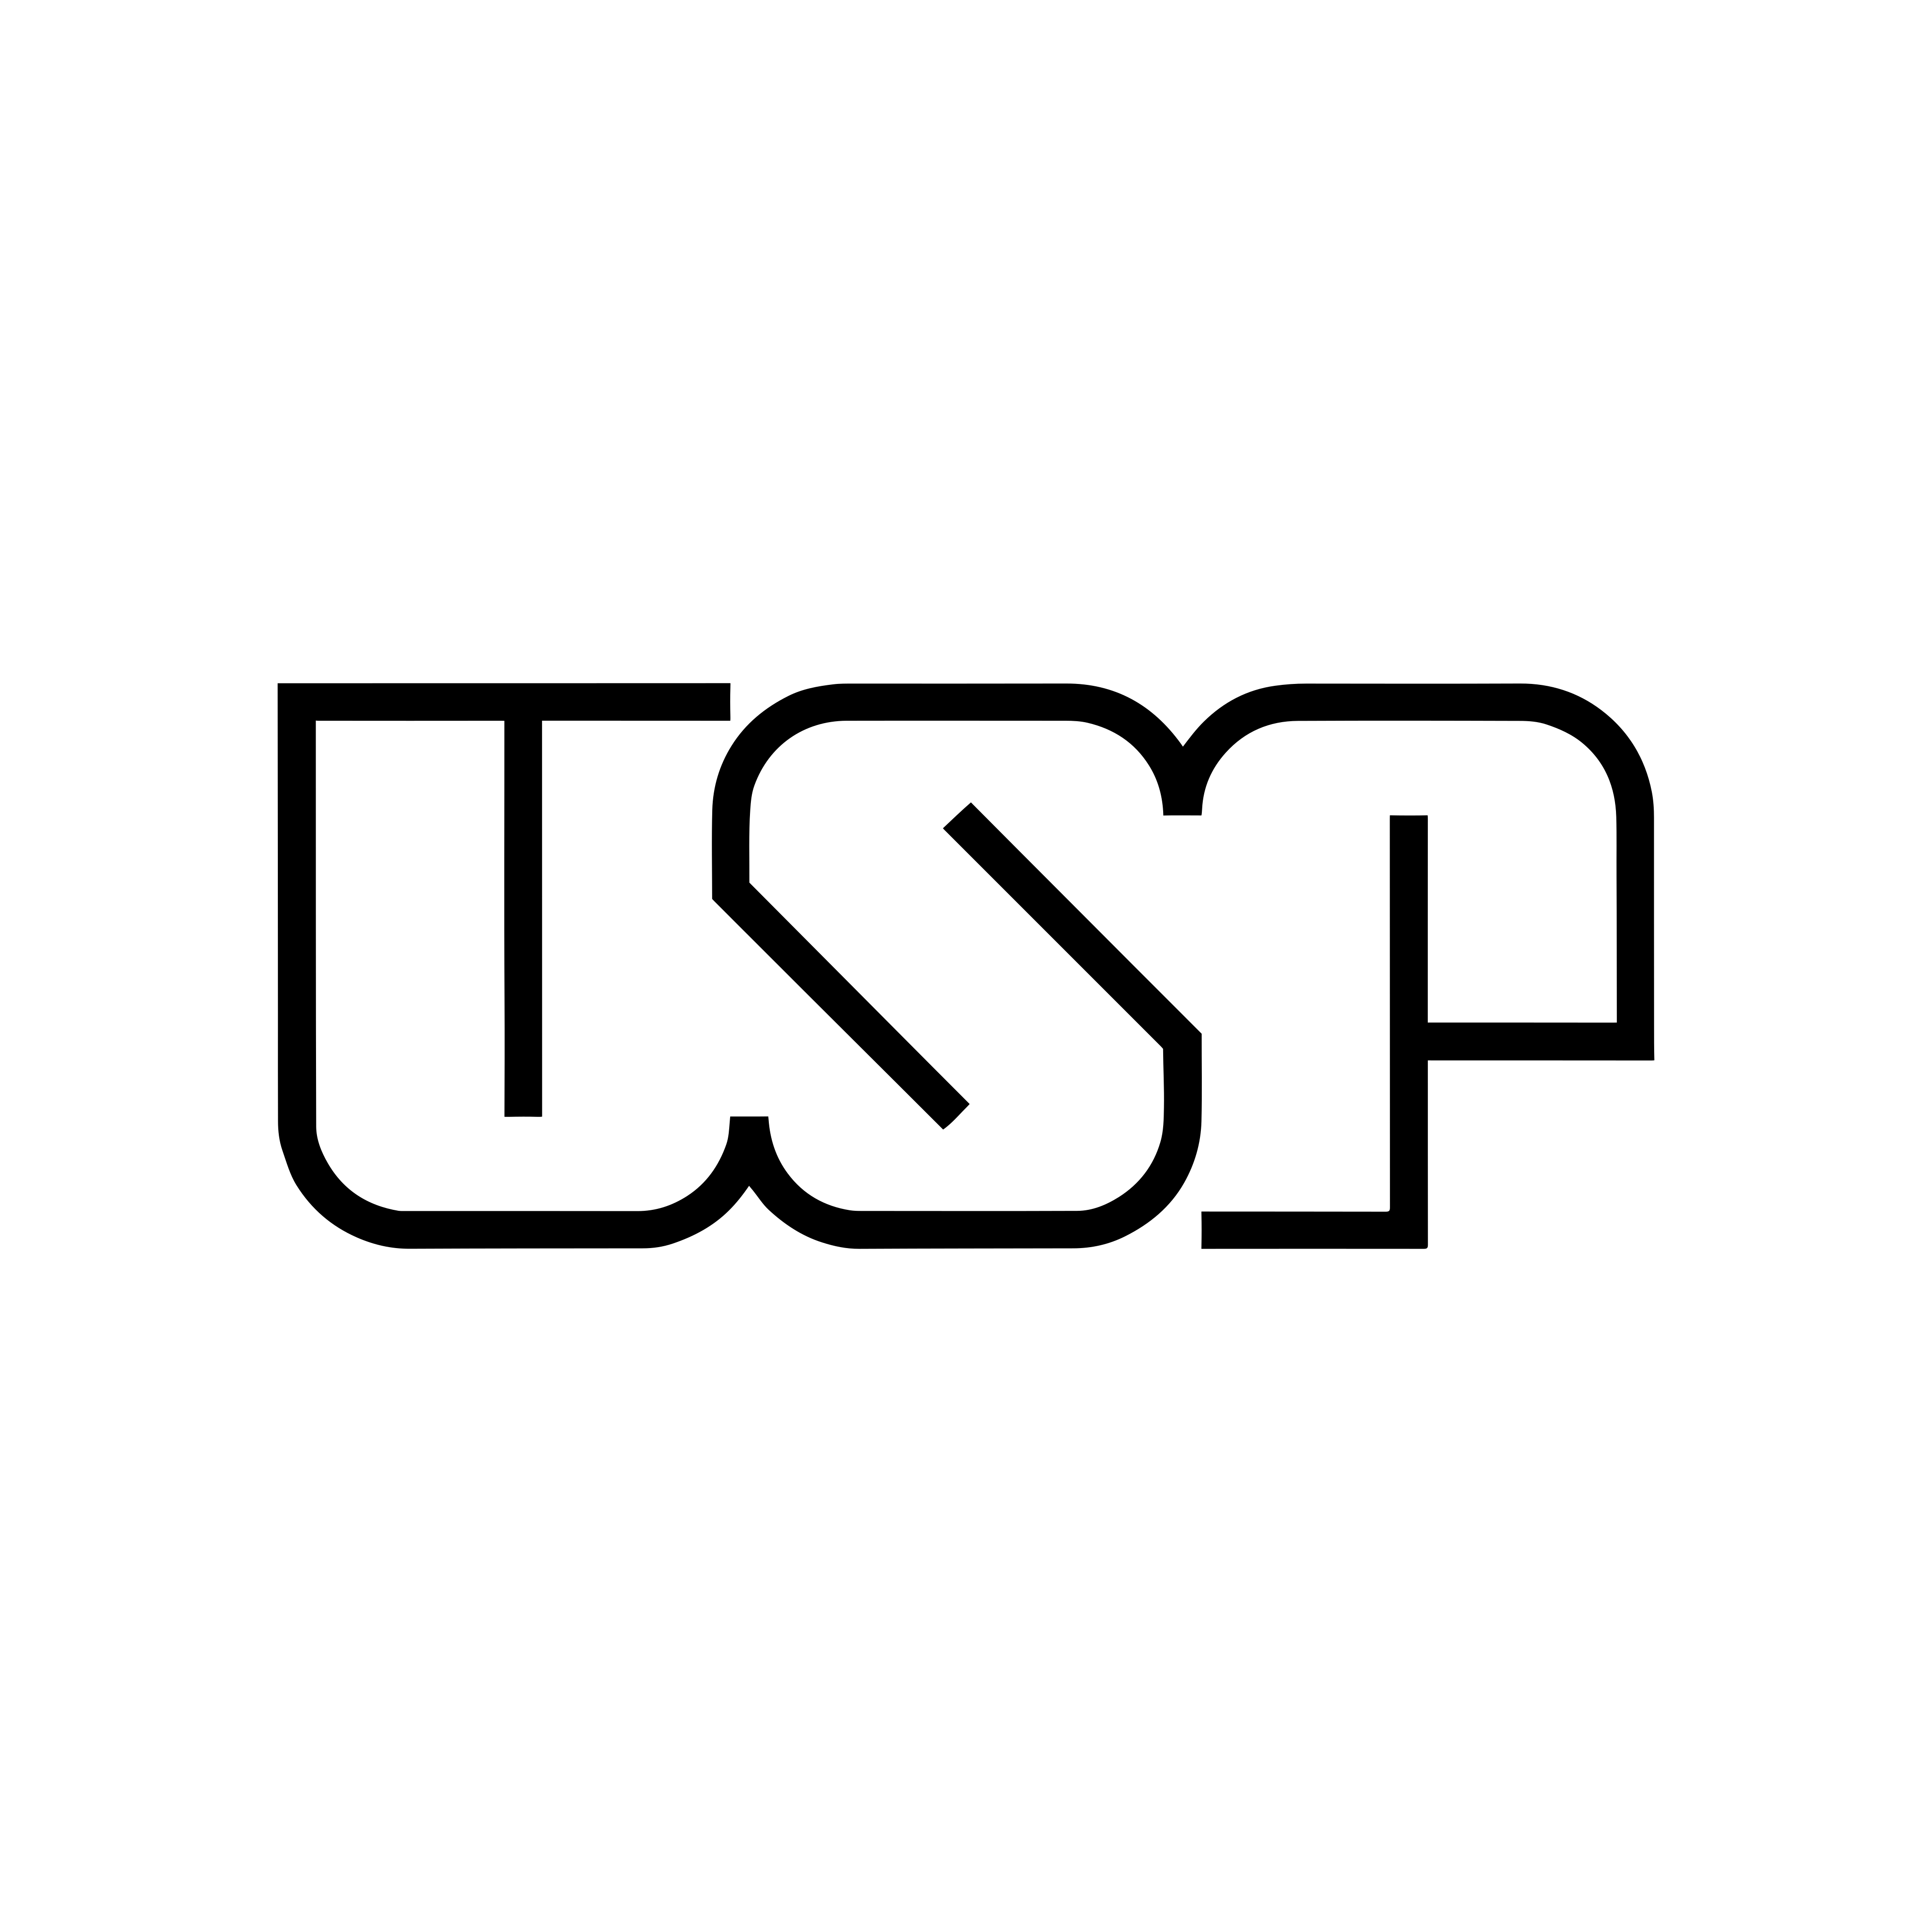
\includegraphics[width=10.0cm]{pags/imagens/usp-logo-0.png} \\[1.5cm]

    {\large \textbf{UNIVERSIDADE DE SÃO PAULO}} \\[0.3cm]
    {\large \textbf{DEPARTAMENTO DE ENGENHARIA MECÂNICA}} \\[0.3cm]
    {\large \textbf{LABORATÓRIO DE FÍSICA EXPERIMENTAL II}} \\[1cm]
    {\Large \textbf{Prática 3: Oscilações livres, amortecidas e forçadas}} \\[0.4cm]
    {\large \textbf{PROFESSOR: Hai Guoqiang}} \\[1cm]
    {\large \textbf{INTEGRANTES:\\}
    Flávio Henrique Monteiro Silva - 17890005 \\ 
    Guilherme Tommasino Ribeiro - 17894232 \\
    Leonardo Miranda de Almeida Prado - 17905098}
    \vfill 
    {\large São Carlos-SP} \\[0.2cm]
    {\large \textbf{2026}}
\end{titlepage}
\clearpage


\setcounter{page}{2}
\thispagestyle{empty}
\tableofcontents
\clearpage

\pagestyle{abnt}
% ======================== pags/1-Introducao_e_Objetivos.tex ========================
\section{Introdução e Objetivos}

\subsection{Introdução}

Diversos fenômenos da natureza se repetem ao longo do tempo, e esses movimentos repetitivos recebem o nome de oscilações. Todo corpo que executa um movimento de vaivém em torno de uma posição de equilíbrio é denominado oscilador e, quando a força restauradora é proporcional ao deslocamento, tem-se um oscilador harmônico\cita{3}.

No sistema massa-mola vertical, a posição de equilíbrio é aquela em que a força elástica da mola compensa o peso do corpo suspenso. Quando o corpo é afastado desse ponto e o meio é pouco dissipativo, como o ar, o sistema se comporta aproximadamente como um oscilador livre, com frequência angular natural $\omega_0=\sqrt{k/m}$, em que $k$ é a constante elástica da mola e $m$ é a massa suspensa\cita{2}. Em um meio viscoso, como a água, a força de atrito viscoso faz com que a amplitude decaia exponencialmente no tempo e a frequência de oscilação diminua para um valor $\omega_1<\omega_0$. Por fim, quando uma força externa periódica de frequência angular $\Omega$ atua sobre o sistema, a massa passa a oscilar com essa frequência, e a amplitude torna-se função de $\Omega$, atingindo um máximo na chamada frequência de ressonância $\Omega_r$\cita{1}.

\subsection{Objetivos}

Este relatório tem como objetivo estudar o comportamento de um oscilador massa-mola vertical quanto à amplitude e à frequência das oscilações, em função da viscosidade do meio (ar e água), nas condições de oscilação livre, amortecida e forçada. Especificamente, busca-se:
\begin{itemize}
    \item determinar as frequências angulares de oscilação no ar ($\omega_0$) e na água ($\omega_1$) e a constante elástica $k$ da mola;
    \item determinar o fator de amortecimento $\gamma$ na água a partir do decaimento das amplitudes e verificar sua consistência com o modelo teórico;
    \item estudar o fenômeno da ressonância na oscilação forçada, determinando $\Omega_r$ no ar e na água e discutindo o efeito do amortecimento sobre a forma da curva de amplitude e sobre a posição do máximo;
    \item discutir as fontes de erro envolvidas em cada procedimento.
\end{itemize}

% ======================== pags/2-Materiais_e_Metodos.tex ========================
\section{Materiais e Métodos}

\subsection{Instrumentos e Materiais}

Para a realização do experimento, foram utilizados os seguintes instrumentos:
\begin{itemize}
    \item Sistema massa-mola vertical montado em suporte, com régua graduada em centímetros para leitura das posições;
    \item Corpo de massa $m$ suspenso na extremidade da mola;
    \item Balança de precisão (resolução de $0{,}01\un{g}$);
    \item Cronômetro digital (resolução de $0{,}01\un{s}$);
    \item Proveta com água;
    \item Sistema de excitação composto por motor elétrico de rotação variável, disco girante e alavanca acoplada ao ponto de suspensão da mola.
\end{itemize}

\subsection{Métodos}

Para uma melhor compreensão do procedimento experimental, além de melhorar a concepção cronológica das práticas, esta seção do relatório será dividida em cinco experimentos diferentes:
\begin{itemize}
    \item Determinação do período e da frequência angular de oscilação do sistema no ar (experimento 1);
    \item Determinação do período e da frequência angular de oscilação do sistema na água (experimento 2);
    \item Análise do decaimento da amplitude da oscilação amortecida na água e determinação do fator de amortecimento (experimento 3);
    \item Estudo da oscilação forçada no ar e determinação da frequência de ressonância (experimento 4);
    \item Estudo da oscilação forçada na água e determinação da frequência de ressonância (experimento 5).
\end{itemize}

Antes dos experimentos, a massa do corpo suspenso foi medida três vezes na balança. As equações utilizadas em cada experimento, apresentadas na apostila da disciplina\cita{1}, são deduzidas a partir da segunda lei de Newton\cita{2,3} à medida que aparecem.

\subsubsection{Experimento 1}

O sistema massa-mola foi posto para oscilar no ar, situação mais próxima de um oscilador livre. A massa foi deslocada para baixo da posição de equilíbrio e solta a partir do repouso, e o tempo de 10 oscilações completas foi medido com o cronômetro. Cronometrar 10 oscilações, em vez de uma única, reduz a incerteza relativa do período, já que o erro associado ao tempo de reação do operador é distribuído por 10 períodos. O procedimento foi repetido cinco vezes.

Como o atrito com o ar é pequeno, o sistema pode ser tratado como um oscilador harmônico livre. Na posição de equilíbrio, a mola está alongada de $\Delta$, de modo que a força elástica compensa o peso, $k\Delta=mg$. Tomando essa posição como origem ($x=0$) e o eixo $x$ orientado para baixo, um deslocamento $x$ da massa resulta na força resultante $mg-k(\Delta+x)=-kx$. O peso, portanto, apenas desloca a posição de equilíbrio, e a segunda lei de Newton fornece
\[
m\frac{d^2x}{dt^2}=-kx
\quad\Longrightarrow\quad
\frac{d^2x}{dt^2}+\frac{k}{m}\,x=0.
\]
A solução geral dessa equação é $x(t)=A\cos(\omega_0 t)+B\sin(\omega_0 t)$, o que se verifica derivando-a duas vezes, $\dfrac{d^2x}{dt^2}=-\omega_0^2x$, e substituindo na equação, desde que
\begin{equation}
\omega_0=\sqrt{\frac{k}{m}},
\label{eq:w0}
\end{equation}
que é a frequência angular natural do sistema. Para a massa solta do repouso em $x=x_0$, isto é, $x(0)=x_0$ e $\dfrac{dx}{dt}(0)=0$, obtém-se $A=x_0$ e $B=0$, logo
\[
x(t)=x_0\cos(\omega_0 t).
\]
O movimento se repete após um período $T$ tal que $\omega T=2\pi$, de modo que a frequência angular é obtida do período medido por
\begin{equation}
\omega=\frac{2\pi}{T}.
\label{eq:wT}
\end{equation}
Com a massa medida, a constante elástica da mola é obtida elevando a Equação~\eqref{eq:w0} ao quadrado e isolando $k$:
\begin{equation}
k=m\,\omega_0^2=\frac{4\pi^2m}{T_0^2}.
\label{eq:k}
\end{equation}

\subsubsection{Experimento 2}

O mesmo sistema foi posicionado de modo que o corpo ficasse dentro da proveta com água, tomando-se o cuidado para que permanecesse sempre submerso e não encostasse nas paredes da proveta. De modo análogo ao Experimento 1, mediu-se cinco vezes o tempo de 10 oscilações, obtendo-se o período $T_1$ e, pela Equação~\eqref{eq:wT}, a frequência angular $\omega_1$, posteriormente comparada com $\omega_0$.

Na água, o amortecimento não pode ser desprezado, e acrescenta-se a força de atrito viscoso, proporcional à velocidade e de sentido oposto a ela:
\[
F_a=-b\,\frac{dx}{dt},
\]
em que $b$ é uma constante que caracteriza o grau de amortecimento. A segunda lei de Newton resulta em
\[
m\frac{d^2x}{dt^2}=-kx-b\frac{dx}{dt}
\quad\Longrightarrow\quad
\frac{d^2x}{dt^2}+2\gamma\frac{dx}{dt}+\omega_0^2x=0,
\qquad
\gamma=\frac{b}{2m},
\]
em que $\gamma$ é o fator de amortecimento. Procurando soluções da forma $x=e^{\lambda t}$, tem-se $\dfrac{dx}{dt}=\lambda x$ e $\dfrac{d^2x}{dt^2}=\lambda^2x$, e a equação se reduz a $\lambda^2+2\gamma\lambda+\omega_0^2=0$, cujas raízes são
\[
\lambda=-\gamma\pm\sqrt{\gamma^2-\omega_0^2}.
\]
Para amortecimento fraco ($\gamma<\omega_0$), a raiz quadrada é imaginária e $\lambda=-\gamma\pm i\,\omega_1$, com
\begin{equation}
\omega_1=\sqrt{\omega_0^2-\gamma^2}.
\label{eq:w1}
\end{equation}
Pela consistência dimensional dessa equação, a unidade de $\gamma$ é rad/s. A Equação~\eqref{eq:w1} mostra que a frequência na água deve ser menor que no ar ($\omega_1<\omega_0$) e, isolando $\gamma$, permite estimar o fator de amortecimento pelas frequências medidas:
\begin{equation}
\gamma=\sqrt{\omega_0^2-\omega_1^2}.
\label{eq:gw}
\end{equation}
Ela mostra ainda que só há oscilação para $\gamma<\omega_0$. Em $\gamma=\omega_0$ (amortecimento crítico), o sistema retorna ao equilíbrio sem oscilar; para $\gamma>\omega_0$ (amortecimento supercrítico), também não há oscilação, e o retorno ao equilíbrio é mais lento que no caso crítico.

\subsubsection{Experimento 3}

Com o corpo ainda na água, a massa foi deslocada até uma amplitude inicial $x_0$ e solta a partir do repouso, sempre da mesma posição inicial. Registrou-se, na régua, a leitura $y_n$ da posição extrema da massa nos instantes $t_n=n\,T_1/2$ ($n=0,1,\dots,6$), isto é, de $t=0$ até $t=3T_1$, em que $T_1$ é o período obtido no Experimento 2. A posição de equilíbrio correspondeu à leitura $y_{eq}=70\un{cm}$, e a amplitude foi definida como $|x_n|=|y_n-y_{eq}|$. O procedimento foi realizado duas vezes.

Para relacionar as amplitudes com $\gamma$, retoma-se a solução do Experimento 2. A solução real correspondente às raízes $\lambda=-\gamma\pm i\,\omega_1$ é $x(t)=e^{-\gamma t}\left[C_1\cos(\omega_1 t)+C_2\sin(\omega_1 t)\right]$. Impondo $x(0)=x_0$, obtém-se $C_1=x_0$; impondo $\dfrac{dx}{dt}(0)=0$, obtém-se $C_2=x_0\gamma/\omega_1$, termo desprezível quando o amortecimento é fraco ($\gamma\ll\omega_1$). Assim,
\begin{equation}
x(t)=\left[x_0\,e^{-\gamma t}\right]\cos(\omega_1 t).
\label{eq:xamort}
\end{equation}
A posição oscila com período $T_1=2\pi/\omega_1$, e o termo entre colchetes faz as amplitudes extremas decrescerem exponencialmente. Como $\cos(\omega_1t)=\pm1$ nos instantes $t_n=n\,T_1/2$, as amplitudes medidas são $|x_n|=x_0e^{-\gamma t_n}$ e, aplicando o logaritmo natural,
\begin{equation}
\ln\left|\frac{x_n}{x_0}\right|=-\gamma\,t_n.
\label{eq:ln}
\end{equation}
Assim, $\ln|x_n/x_0|$ varia linearmente com $t_n$, e $\gamma$ foi determinado como o oposto do coeficiente angular da regressão linear desses dados.

\subsubsection{Experimento 4}

Com o corpo oscilando no ar, ligou-se o motor que desloca periodicamente o ponto de suspensão da mola. Para diferentes rotações do motor, aguardou-se o término do regime transitório e mediu-se, na régua, a amplitude máxima $x_0$ de oscilação da massa. A frequência de excitação foi determinada cronometrando-se o tempo $t_7$ de 7 rotações do disco, de modo que $\Omega=2\pi\cdot7/t_7$. Foram escolhidas frequências abaixo, acima e próximas da ressonância, e, na condição de ressonância, na qual a amplitude cresceu consideravelmente, o tempo de 7 rotações foi medido duas vezes.

O motor exerce sobre o sistema uma força externa harmônica $F_{ext}=F_0\cos(\Omega t)$, em que $\Omega$ é a frequência angular imposta e $F_0$ é sua amplitude. A segunda lei de Newton fornece
\[
m\frac{d^2x}{dt^2}=-kx-b\frac{dx}{dt}+F_0\cos(\Omega t)
\quad\Longrightarrow\quad
\frac{d^2x}{dt^2}+2\gamma\frac{dx}{dt}+\omega_0^2x=\frac{F_0}{m}\cos(\Omega t).
\]
Após o regime transitório, que decai como $e^{-\gamma t}$, a massa oscila com a frequência imposta:
\[
x(t)=x_0(\Omega)\cos(\Omega t+\delta),
\]
em que $\delta$ é uma constante de fase que não será discutida nesta prática. Para determinar $x_0(\Omega)$, escreve-se $x(t)$ como a parte real de $X e^{i\Omega t}$, com $X=x_0e^{i\delta}$, e a força como a parte real de $F_0e^{i\Omega t}$. Como $\dfrac{d}{dt}e^{i\Omega t}=i\Omega\,e^{i\Omega t}$ e $\dfrac{d^2}{dt^2}e^{i\Omega t}=-\Omega^2e^{i\Omega t}$, a substituição na equação diferencial resulta em
\[
\left(\omega_0^2-\Omega^2+2i\gamma\Omega\right)X=\frac{F_0}{m},
\]
cujo módulo fornece a amplitude
\begin{equation}
x_0(\Omega)=\frac{F_0/m}{\sqrt{\left(\omega_0^2-\Omega^2\right)^2+4\gamma^2\Omega^2}}.
\label{eq:x0W}
\end{equation}
A amplitude independe do tempo e depende da frequência da força externa. O máximo de $x_0(\Omega)$ ocorre quando o radicando $D(\Omega)=\left(\omega_0^2-\Omega^2\right)^2+4\gamma^2\Omega^2$ é mínimo:
\[
\frac{dD}{d\Omega}=-4\Omega\left(\omega_0^2-\Omega^2\right)+8\gamma^2\Omega
=4\Omega\left(\Omega^2-\omega_0^2+2\gamma^2\right)=0,
\]
cuja solução não nula é a frequência de ressonância
\begin{equation}
\Omega_r=\sqrt{\omega_0^2-2\gamma^2}.
\label{eq:Wr}
\end{equation}
Para amortecimento nulo ($\gamma=0$), $\Omega_r=\omega_0$ e $x_0(\Omega)$ tende ao infinito na ressonância. Como, na realidade, $\gamma\neq0$, a amplitude permanece finita. No ar, em que $\gamma$ é pequeno, espera-se $\Omega_r\approx\omega_0$ e amplitudes muito grandes perto da ressonância.

\subsubsection{Experimento 5}

O procedimento do Experimento 4 foi repetido com o corpo oscilando dentro da proveta com água, medindo-se a amplitude máxima $x_0$ para diferentes valores de $\Omega$, inclusive na condição de ressonância, em que o tempo de 7 rotações foi cronometrado duas vezes. Os valores de $x_0(\Omega)$ obtidos no ar e na água foram então comparados.

Pelas Equações~\eqref{eq:x0W} e \eqref{eq:Wr}, o aumento de $\gamma$ na água deve reduzir a amplitude máxima, tornar a variação de $x_0$ com $\Omega$ mais suave em torno do máximo e deslocar a frequência de ressonância para valores menores que $\omega_0$.

% ======================== pags/3-Resultados_experimentais.tex ========================
\section{Resultados e Discussões}

Para as grandezas medidas repetidamente, adotou-se como resultado a média e, como incerteza, o desvio-padrão amostral das medidas,
\[
s=\sqrt{\frac{1}{N-1}\sum_{i=1}^{N}\left(q_i-\bar{q}\right)^2}.
\]

\subsection{Oscilação no ar e constante elástica da mola}

A massa do corpo foi medida três vezes, obtendo-se $10{,}90$, $10{,}91$ e $10{,}70\un{g}$, de modo que
\[
m=\frac{10{,}90+10{,}91+10{,}70}{3}=(10{,}84\pm0{,}12)\un{g}.
\]

A Tabela~\ref{tab:ar} apresenta os tempos de 10 oscilações medidos no ar, os períodos $T=t_{10}/10$, as frequências angulares obtidas pela Equação~\eqref{eq:wT} e as constantes elásticas obtidas pela Equação~\eqref{eq:k}, calculadas com a massa média.

\begin{table}[H]
\centering
\caption{Período, frequência angular e constante elástica para a oscilação no ar.}
\label{tab:ar}
\begin{tabular}{ccccc}
\toprule
Medida & $t_{10}$ (s) & $T_0$ (s) & $\omega_0$ (rad/s) & $k$ (N/m) \\
\midrule
1 & 13,91 & 1,391 & 4,517 & 0,2211 \\
2 & 13,99 & 1,399 & 4,491 & 0,2186 \\
3 & 14,04 & 1,404 & 4,475 & 0,2170 \\
4 & 13,97 & 1,397 & 4,498 & 0,2192 \\
5 & 14,02 & 1,402 & 4,482 & 0,2177 \\
\midrule
Média & --- & 1,399 & 4,493 & 0,2187 \\
Desvio-padrão & --- & 0,005 & 0,016 & 0,0016 \\
\bottomrule
\end{tabular}
\fonte{Elaborada pelos autores.}
\end{table}

Para a medida 1, por exemplo,
\[
\omega_0=\frac{2\pi}{1{,}391}=4{,}517\un{rad/s},
\qquad
k=\frac{4\pi^2\left(10{,}84\times10^{-3}\right)}{(1{,}391)^2}=0{,}2211\un{N/m}.
\]
Assim, o período de oscilação no ar, a frequência angular natural e a constante elástica da mola são
\[
T_0=(1{,}399\pm0{,}005)\un{s},
\qquad
\omega_0=(4{,}493\pm0{,}016)\un{rad/s},
\qquad
k=(0{,}219\pm0{,}002)\un{N/m}.
\]

\subsection{Oscilação na água: análise do período}

A Tabela~\ref{tab:agua} mostra os tempos de 10 oscilações, os períodos e as frequências angulares obtidos com o corpo oscilando na água.

\begin{table}[H]
\centering
\caption{Período e frequência angular para a oscilação na água.}
\label{tab:agua}
\begin{tabular}{cccc}
\toprule
Medida & $t_{10}$ (s) & $T_1$ (s) & $\omega_1$ (rad/s) \\
\midrule
1 & 14,60 & 1,460 & 4,304 \\
2 & 14,24 & 1,424 & 4,412 \\
3 & 14,13 & 1,413 & 4,447 \\
4 & 14,36 & 1,436 & 4,376 \\
5 & 14,27 & 1,427 & 4,403 \\
\midrule
Média & --- & 1,432 & 4,388 \\
Desvio-padrão & --- & 0,018 & 0,054 \\
\bottomrule
\end{tabular}
\fonte{Elaborada pelos autores.}
\end{table}

Logo,
\[
T_1=(1{,}432\pm0{,}018)\un{s},
\qquad
\omega_1=(4{,}388\pm0{,}054)\un{rad/s}.
\]

Comparando com o valor no ar, a frequência diminuiu $0{,}105\un{rad/s}$, ou seja, $2{,}3\%$. Os intervalos $\omega_0=[4{,}477;\,4{,}509]\un{rad/s}$ e $\omega_1=[4{,}334;\,4{,}442]\un{rad/s}$ não se sobrepõem, de modo que se pode afirmar que as frequências são diferentes. O sentido da diferença ($\omega_1<\omega_0$) é coerente com a Equação~\eqref{eq:w1}, que prevê frequência menor na presença de amortecimento. Pela Equação~\eqref{eq:gw}, o fator de amortecimento correspondente seria
\[
\gamma=\sqrt{(4{,}493)^2-(4{,}388)^2}=\sqrt{20{,}183-19{,}257}=0{,}96\un{rad/s},
\]
valor comparado, na próxima seção, com o obtido pelo decaimento das amplitudes.

\subsection{Oscilação na água: análise da variação de amplitude}

Com $T_1=1{,}432\un{s}$, os instantes de medida $t_n=n\,T_1/2$ são $0$; $0{,}716$; $1{,}432$; $2{,}148$; $2{,}864$; $3{,}580$ e $4{,}296\un{s}$. A Tabela~\ref{tab:decaimento} apresenta as amplitudes $|x_n|=|y_n-y_{eq}|$ medidas nas duas realizações do experimento, que resultaram em valores iguais, as amplitudes normalizadas por $x_0=15{,}0\un{cm}$ e seus logaritmos.

\begin{table}[H]
\centering
\caption{Amplitude de oscilação na água em função do tempo.}
\label{tab:decaimento}
\begin{tabular}{cccccc}
\toprule
$n$ & $t_n$ (s) & $|x_n|$ -- 1.ª medida (cm) & $|x_n|$ -- 2.ª medida (cm) & $|x_n/x_0|$ & $\ln|x_n/x_0|$ \\
\midrule
0 & 0,000 & 15,0 & 15,0 & 1,000 & $0{,}000$ \\
1 & 0,716 & 10,0 & 10,0 & 0,667 & $-0{,}405$ \\
2 & 1,432 & 7,0 & 7,0 & 0,467 & $-0{,}762$ \\
3 & 2,148 & 5,5 & 5,5 & 0,367 & $-1{,}003$ \\
4 & 2,864 & 4,5 & 4,5 & 0,300 & $-1{,}204$ \\
5 & 3,580 & 3,5 & 3,5 & 0,233 & $-1{,}455$ \\
6 & 4,296 & 3,0 & 3,0 & 0,200 & $-1{,}609$ \\
\bottomrule
\end{tabular}
\fonte{Elaborada pelos autores.}
\end{table}

As amplitudes decrescem progressivamente, e $\ln|x_n/x_0|$ diminui de forma aproximadamente linear com $t_n$, o que indica um decaimento exponencial, consistente com as Equações~\eqref{eq:xamort} e \eqref{eq:ln}. A regressão linear de $\ln|x_n/x_0|$ em função de $t_n$ resultou em coeficiente angular $-0{,}368\un{rad/s}$, com desvio-padrão $0{,}025\un{rad/s}$, coeficiente linear $-0{,}13$ e coeficiente de correlação $r=-0{,}988$. Portanto,
\[
\gamma=(0{,}37\pm0{,}03)\un{rad/s}.
\]
O coeficiente linear, que pela Equação~\eqref{eq:ln} deveria ser nulo, e a leve curvatura dos dados, com decaimento mais rápido no início do movimento, indicam que o modelo exponencial é apenas aproximado.

O decaimento das amplitudes mostra também que a energia mecânica do oscilador não se conserva. Nos pontos extremos a velocidade é nula e a energia é apenas potencial elástica, $E_n=\frac{1}{2}k\,x_n^2=\frac{1}{2}k\,x_0^2e^{-2\gamma t_n}$, de modo que a energia decai exponencialmente, sendo dissipada pelo atrito viscoso. Ao final de $3T_1$, por exemplo, $(x_6/x_0)^2=(0{,}200)^2=0{,}04$, isto é, restavam apenas $4\%$ da energia inicial.

Para verificar a consistência com a Equação~\eqref{eq:w1}, calculou-se o valor previsto de $\omega_1$ com o $\gamma$ obtido do decaimento:
\[
\omega_1=\sqrt{(4{,}493)^2-(0{,}37)^2}=4{,}477\un{rad/s},
\]
valor fora do intervalo medido, $\omega_1=(4{,}388\pm0{,}054)\un{rad/s}$. De forma equivalente, o valor $\gamma=0{,}96\un{rad/s}$, obtido na seção anterior a partir de $\omega_0$ e $\omega_1$, é cerca de 2,6 vezes maior que o obtido pelo decaimento. Portanto, os resultados não são estritamente consistentes com a Equação~\eqref{eq:w1}. Algumas causas plausíveis são:
\begin{enumerate}
    \item a frequência $\omega_0$ foi medida no ar, mas, na água, o corpo arrasta fluido consigo, o que aumenta sua massa efetiva e reduz a frequência natural no meio; assim, a Equação~\eqref{eq:gw}, aplicada com o $\omega_0$ do ar, atribui ao amortecimento uma redução de frequência que se deve, em parte, à massa efetiva, superestimando $\gamma$;
    \item o valor de $\gamma$ obtido pela Equação~\eqref{eq:gw} resulta da diferença entre dois números muito próximos ($20{,}18$ e $19{,}26\un{rad^2/s^2}$), o que o torna muito sensível a pequenos erros de cronometragem;
    \item a curvatura observada nos dados da Tabela~\ref{tab:decaimento} sugere que a força de atrito não é puramente proporcional à velocidade, de modo que o ajuste por uma única exponencial é aproximado;
    \item as amplitudes foram lidas visualmente na régua com a massa em movimento e nos instantes $t_n$ estimados pelo operador.
\end{enumerate}

\subsection{Oscilação forçada no ar}

Para cada rotação do motor, a frequência de excitação foi calculada por $\Omega=2\pi\cdot7/t_7$. Observa-se que os valores $7/t_7$ anotados no laboratório correspondem a rotações por segundo (Hz), sendo necessária a multiplicação por $2\pi$ para obter $\Omega$ em rad/s. A Tabela~\ref{tab:forcada_ar} reúne os dados obtidos.

\begin{table}[H]
\centering
\caption{Amplitude máxima da oscilação forçada no ar em função da frequência de excitação.}
\label{tab:forcada_ar}
\begin{tabular}{ccccc}
\toprule
Ponto & $t_7$ (s) & $7/t_7$ (Hz) & $\Omega$ (rad/s) & $x_0$ (cm) \\
\midrule
1 & 19,16 & 0,365 & 2,296 & 10,7 \\
2 & 12,56 & 0,557 & 3,502 & 21,4 \\
3 & 10,46 & 0,669 & 4,205 & 49,0 \\
R & 9,73 & 0,719 & 4,520 & $>49{,}0$ (não medida) \\
4 & 6,79 & 1,031 & 6,478 & 9,8 \\
5 & 4,03 & 1,737 & 10,914 & 8,3 \\
6 & 3,63 & 1,928 & 12,116 & 3,3 \\
\bottomrule
\end{tabular}
\fonte{Elaborada pelos autores.}
\end{table}

A amplitude cresce à medida que $\Omega$ se aproxima da ressonância e decai rapidamente acima dela. Na condição de ressonância, em que a amplitude ficou grande demais para ser medida, mediram-se $t_7=9{,}74\un{s}$ e $t_7=9{,}72\un{s}$, que correspondem a
\[
\Omega=\frac{2\pi\cdot7}{9{,}74}=4{,}516\un{rad/s}
\qquad\text{e}\qquad
\Omega=\frac{2\pi\cdot7}{9{,}72}=4{,}525\un{rad/s},
\]
de modo que a frequência de ressonância no ar é
\[
\Omega_R^{ar}=(4{,}520\pm0{,}007)\un{rad/s}.
\]

Comparando com a frequência do oscilador livre, $\omega_0=(4{,}493\pm0{,}016)\un{rad/s}$, a diferença é de $0{,}028\un{rad/s}$, ou seja, $0{,}6\%$. Os valores são, portanto, muito próximos, como esperado para um meio de baixo amortecimento, em que a Equação~\eqref{eq:Wr} fornece $\Omega_r\approx\omega_0$. Estritamente, a Equação~\eqref{eq:Wr} prevê $\Omega_r\le\omega_0$, enquanto o resultado experimental ficou ligeiramente acima, praticamente no limite dos intervalos de incerteza. Essa pequena diferença pode ser atribuída ao tempo de reação do operador ao iniciar e parar o cronômetro e à dificuldade de identificar visualmente a rotação exata em que a amplitude é máxima. Mesmo que o amortecimento no ar fosse tão grande quanto o medido na água ($\gamma=0{,}37\un{rad/s}$), a Equação~\eqref{eq:Wr} preveria $\Omega_r=4{,}462\un{rad/s}$, uma redução de apenas $0{,}7\%$ em relação a $\omega_0$.

\subsection{Oscilação forçada na água}

De modo análogo, os dados obtidos com o corpo na água estão na Tabela~\ref{tab:forcada_agua}.

\begin{table}[H]
\centering
\caption{Amplitude máxima da oscilação forçada na água em função da frequência de excitação.}
\label{tab:forcada_agua}
\begin{tabular}{ccccc}
\toprule
Ponto & $t_7$ (s) & $7/t_7$ (Hz) & $\Omega$ (rad/s) & $x_0$ (cm) \\
\midrule
1 & 22,30 & 0,314 & 1,972 & 7,5 \\
2 & 13,34 & 0,525 & 3,297 & 12,7 \\
3 & 11,63 & 0,602 & 3,782 & 19,0 \\
R & 10,445 & 0,670 & 4,211 & 22,9 \\
4 & 8,67 & 0,807 & 5,073 & 14,7 \\
5 & 7,77 & 0,901 & 5,661 & 8,2 \\
6 & 6,02 & 1,163 & 7,306 & 4,2 \\
\bottomrule
\end{tabular}
\fonte{Elaborada pelos autores.}
\end{table}

Na ressonância, mediram-se $t_7=10{,}52\un{s}$ e $t_7=10{,}37\un{s}$, que correspondem a $\Omega=4{,}181\un{rad/s}$ e $\Omega=4{,}241\un{rad/s}$. Assim,
\[
\Omega_R^{ag}=(4{,}21\pm0{,}04)\un{rad/s},
\]
com amplitude máxima $x_0=22{,}9\un{cm}$.

Comparando as Tabelas~\ref{tab:forcada_ar} e \ref{tab:forcada_agua}, nota-se que, no ar, a amplitude cresce muito perto da ressonância: já em $\Omega=4{,}205\un{rad/s}$ obteve-se $x_0=49{,}0\un{cm}$, e na ressonância a amplitude ultrapassou a faixa mensurável. Na água, o máximo foi de apenas $22{,}9\un{cm}$, e a amplitude varia de forma mais suave em torno de $\Omega_R$. Isso é coerente com a Equação~\eqref{eq:x0W}: quanto maior o fator de amortecimento, menor a amplitude máxima e mais larga a curva de ressonância. Quanto à posição do máximo, $\Omega_R$ diminuiu de $4{,}520\un{rad/s}$ no ar para $4{,}21\un{rad/s}$ na água, uma redução de $6{,}8\%$, também no sentido previsto pela Equação~\eqref{eq:Wr}, em que o aumento de $\gamma$ desloca a ressonância para frequências menores.

A consistência quantitativa com a Equação~\eqref{eq:Wr} depende do valor de $\gamma$ adotado, como mostra a Tabela~\ref{tab:comparacao}.

\begin{table}[H]
\centering
\caption{Valores de $\Omega_r$ na água previstos pela Equação~\eqref{eq:Wr}, com $\omega_0=4{,}493\un{rad/s}$.}
\label{tab:comparacao}
\begin{tabular}{lcc}
\toprule
Origem de $\gamma$ & $\gamma$ (rad/s) & $\Omega_r$ prevista (rad/s) \\
\midrule
Decaimento da amplitude (Equação~\ref{eq:ln}) & 0,37 & 4,462 \\
Frequências $\omega_0$ e $\omega_1$ (Equação~\ref{eq:gw}) & 0,96 & 4,282 \\
\midrule
Valor experimental & --- & $4{,}21\pm0{,}04$ \\
\bottomrule
\end{tabular}
\fonte{Elaborada pelos autores.}
\end{table}

Ambas as previsões indicam diminuição de $\Omega_r$ em relação a $\omega_0$, mas ficam acima do valor experimental. O deslocamento observado ($6{,}3\%$ abaixo de $\omega_0$) é bem maior que o previsto com $\gamma=0{,}37\un{rad/s}$ ($0{,}7\%$) e mais próximo da previsão com $\gamma=0{,}96\un{rad/s}$. Isso reforça que o modelo de atrito viscoso linear, com $\omega_0$ igual ao do ar, descreve o sistema na água apenas de modo aproximado, sendo o aumento da massa efetiva do corpo pelo fluido arrastado a causa mais provável da diferença, pois reduz a frequência natural na água. Além disso, a ressonância foi identificada por inspeção visual do máximo de amplitude, o que limita a precisão de $\Omega_R$.

% ======================== pags/4-Conclusao.tex ========================
\section{Conclusão}

Os experimentos permitiram observar o comportamento de um oscilador massa-mola vertical em oscilação livre, amortecida e forçada. No ar, o período foi $T_0=(1{,}399\pm0{,}005)\un{s}$, resultando em $\omega_0=(4{,}493\pm0{,}016)\un{rad/s}$ e, com a massa de $(10{,}84\pm0{,}12)\un{g}$, em uma constante elástica $k=(0{,}219\pm0{,}002)\un{N/m}$. Na água, o período aumentou para $T_1=(1{,}432\pm0{,}018)\un{s}$ e a frequência diminuiu para $\omega_1=(4{,}388\pm0{,}054)\un{rad/s}$, diferença no sentido previsto pelo modelo do oscilador amortecido.

As amplitudes na água apresentaram decaimento aproximadamente exponencial, com $\gamma=(0{,}37\pm0{,}03)\un{rad/s}$, evidenciando também a dissipação da energia mecânica pelo atrito. Esse valor, entretanto, não é consistente com o obtido pela relação $\omega_1=\sqrt{\omega_0^2-\gamma^2}$, de $0{,}96\un{rad/s}$, discrepância atribuída principalmente ao aumento da massa efetiva do corpo na água, que reduz a frequência natural em relação à medida no ar, à sensibilidade dessa relação a pequenos erros de cronometragem e ao caráter não puramente linear do atrito.

Na oscilação forçada, a frequência de ressonância no ar, $\Omega_R=(4{,}520\pm0{,}007)\un{rad/s}$, foi muito próxima da frequência natural $\omega_0$ (diferença de $0{,}6\%$), com amplitude muito grande. Na água, a ressonância ocorreu em $\Omega_R=(4{,}21\pm0{,}04)\un{rad/s}$, com amplitude máxima de $22{,}9\un{cm}$, menor e com variação mais suave que no ar, confirmando qualitativamente o efeito do amortecimento sobre a forma da curva e sobre a posição do máximo, previsto por $\Omega_r=\sqrt{\omega_0^2-2\gamma^2}$. Quantitativamente, o deslocamento medido foi maior que o previsto com o $\gamma$ obtido do decaimento, o que reforça que o modelo de atrito viscoso linear é apenas aproximado para o sistema na água.

Assim, a prática permitiu compreender experimentalmente os fenômenos de amortecimento e ressonância e evidenciou a importância da precisão das medidas, sobretudo as de cronometragem e de leitura das amplitudes, para a confiabilidade dos resultados.

% ======================== pags/5-Bibliografia.tex ========================
\section{Bibliografia}

\begin{enumerate}
    \item SCHNEIDER, J. F.; AZEVEDO, E. R. (comp.). \textbf{Laboratório de Física II}: livro de práticas. São Carlos: Instituto de Física de São Carlos, 2018.
    \item HALLIDAY, D.; RESNICK, R.; WALKER, J. \textbf{Fundamentos de física}: gravitação, ondas e termodinâmica. 10. ed. Rio de Janeiro: LTC, 2016. v. 2.
    \item NUSSENZVEIG, H. M. \textbf{Curso de física básica}: fluidos, oscilações e ondas, calor. 5. ed. São Paulo: Blucher, 2014. v. 2.
\end{enumerate}


\end{document}
